% !TeX spellcheck = en_US
\documentclass[letterpaper,12pt,twoside]{report}
\usepackage{fancyhdr}
\usepackage{fullpage}
\usepackage{tikz}
\usepackage{amsmath}

\begin{document}
	\pagestyle{fancy}
	\fancyhf{}
	\fancyhead[L]{Day 6}
	\fancyhead[R]{\textit{The Calendar Project}}
	\fancyfoot[L]{Citations Involved: 1, 2, 3}
	
	% Problem
	\paragraph{Problem}
	\begin{quote}
	\textsf{An equilateral triangle is inscribed in a circle of radius 6 in. A second equilateral triangle is circumscribed about the circle. If the sides of the triangles are parallel, what is the shortest distance from a point on one triangle to a point on the other?}
	\end{quote}
	
	% Graphics
	\begin{center}
		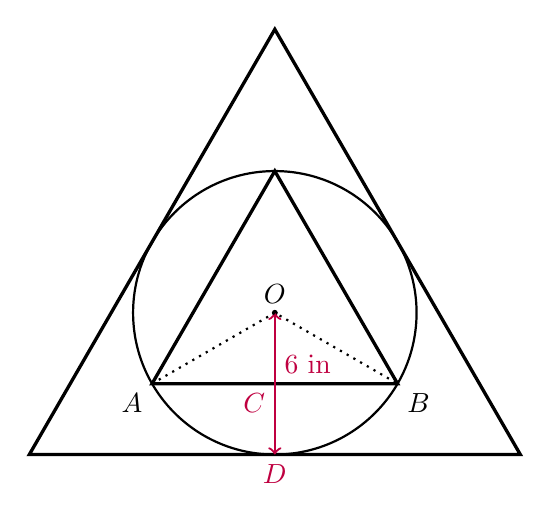
\begin{tikzpicture}[scale=0.3]
		\draw[thick] (0,0) circle [radius=6];
		\draw[very thick] (0,6) -- (-5.19615,-3) -- (5.19615,-3) -- cycle;
		\draw[very thick] (0,12) -- (-10.3923,-6) -- (10.3923,-6) -- cycle;
		
		\draw[fill=black] (0,0) circle [radius=0.1];
		\node[above] at (0,0) {$O$};
		
		\draw[<->][thick][purple] (0,0) -- (0,-6);
		\node[below][purple] at (0,-6) {$D$};
		\node[above right][purple] at (0,-3) {$6$ in};
		\node[below left][purple] at (0,-3) {$C$};
		
		\draw[dotted][thick] (-5.19615,-3) -- (0,0) -- (5.19615,-3);
		\node[below left] at (-5.19615,-3) {$A$};
		\node[below right] at (5.19615,-3) {$B$};
		\end{tikzpicture}
	\end{center}
	
	% Reasoning
	\paragraph{Reasoning}
	\begin{quotation}
	
	The complement of the condition that \textit{``at least 1 six appears''} is that no six appears, which has a probability of $\frac{\textrm{\small{favorable}}}{\textrm{\small{all possible}}} = \frac{5}{6}$ for 1 roll (1). Since it is given that the die is tossed 6 times, and since this negated condition requires \textbf{all} rolls (not just one) to not be six, the cumulative probability for this negated condition is $(\frac{5}{6})^6 = \frac{5^6}{6^6} = \frac{15625}{46656}$ (3). This result's complement, the solution to the problem, is $1-\frac{15625}{46656} = \boxed{\frac{31031}{46656} \approx 0.665}$ (2).
	
	\end{quotation}
	
	\paragraph{External References}
	
	\begin{enumerate}
		\item Textbook Ch. 13, Pg. 878: Theoretical Probability
		\item Textbook Ch. 13, Pg. 879: Complement
		\item Textbook Ch. 13, Pg. 887: Probability of Independent Events
	\end{enumerate}

\end{document}